\section{Scenario}
    We can define four parts of interest for our tool.
    \paragraph{System under test} The system under test is the Erlang system the engineer wishes to observe, it ideally is a system which already is instrumented with OpenTelemetry. The ideal system where $\Delta$QSD is more useful is a system that executes many independent instances of the same action.
    
    \paragraph{Stub/wrapper} The stub is the \texttt{otel\_wrapper}, a wrapper that starts and ends OpenTelemetry spans, and start custom spans which are useful for the oscilloscope. Further handling of OpenTelemetry spans is delegated to the user, who may wish to do further operations with their spans. 
    The custom spans can be ended normally like OpenTelemetry spans or can timeout, given a custom timeout, and fail, according to user's definition of failure. \\
    The stub is called from the system under test and communicates spans data to the oscilloscope via TCP. \\
    The stub can receive messages from the oscilloscope, the messages are about updating observable's $dMax$.
    
    \paragraph{Server} The server is responsible for receiving the messages containing the custom spans from the oscilloscope. The server forwards the spans to the oscilloscope.
    
    \paragraph{Oscilloscope} The oscilloscope receives the custom spans from the stub and creates samples from said spans. \\
    The oscilloscope has a graphical interface which allows the user to create an outcome diagram of the system under test, display real time graphs which show detail about the execution of the system and allow the user to set custom timeouts for observables.

    \begin{figure}[H]
    \begin{center}
        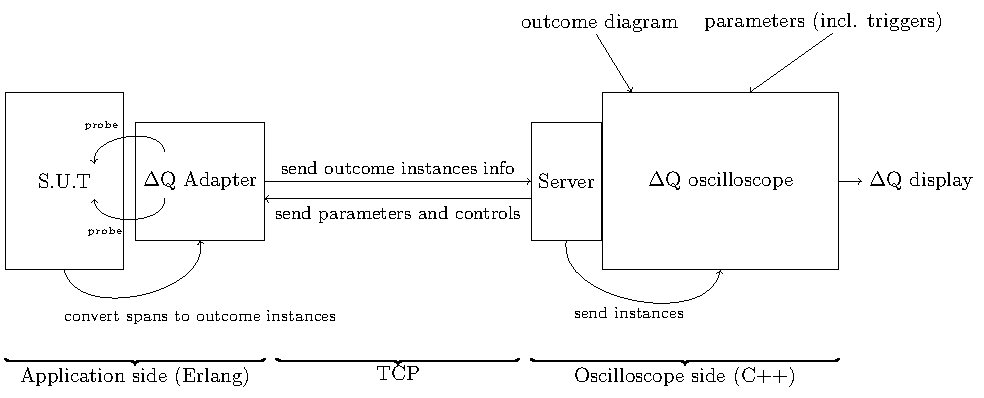
\includegraphics{tikz/sut-stub-osc.pdf}
    \end{center}
    \caption{Global system diagram: the SUT calls the wrapper when starting, ending and failing spans. The spans are received by the server which processes them and sends them to the oscilloscope. The server communicates with the stub to update informations about the system under test ($dMax$)}
    \end{figure}
